\documentclass[Bachelorarbeit.tex]{subfiles}
\begin{document}

\graphicspath{{./figures/topologies/}}	%specifying the folder for the figures

\chapter{Topologies and Hypothesis}
Eigentliche Fragestellung: Wie wichtig ist die Vollvernetzung?
	Allgemeine Netzwerkstrukturen untersuchen aber mit hauptaugenmerk auf Ascending-Connected d.h. reicht ascending-connected aus?


\section{Hypothesis}
hypothese vorstellen: jedes paar von agenten muss über einen kantenzug erreichbar sein, in dem der optimismusfaktor von agent zu agent monoton wächst.


\section{Topologies}
All Topologies are demonstrated with 30 Agents only for better visibility and übersicht of edges. 
All topologies have connected-component of 1 (TODO: warum) except Erdos-Renyi can produce connected-component > 1.

\subsection{Fully-Connected}

\begin{figure}[H]
	\centering
  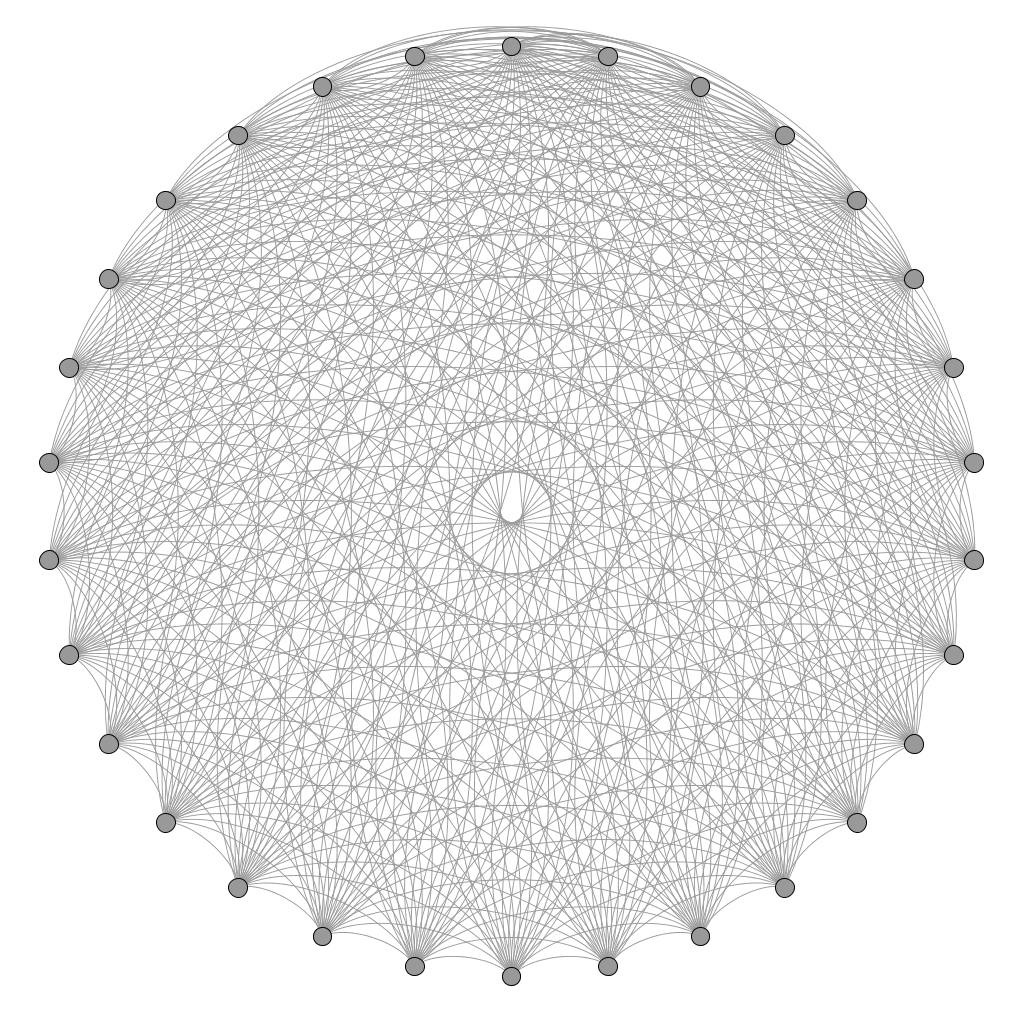
\includegraphics[width=1.0\textwidth, angle=0]{FULLY_CONNECTED_30.png}
	\caption{Fully-Connected topology}
	\label{fig1}
\end{figure}

\begin{table}[h]
	\centering
	\caption{Network metrics Fully-Connected topology}
	\begin{tabular} { l c r }
		\hline
		Avg. degree & 29 \\
		Avg. path-length & 1 \\
		Avg. clustering coefficient & 1 \\
		Network diameter & 1 \\
		Graph density & 1 \\
		\hline
	\end{tabular}
\end{table}

\subsection{Half-Fully Connected}
\begin{figure}[H]
	\centering
  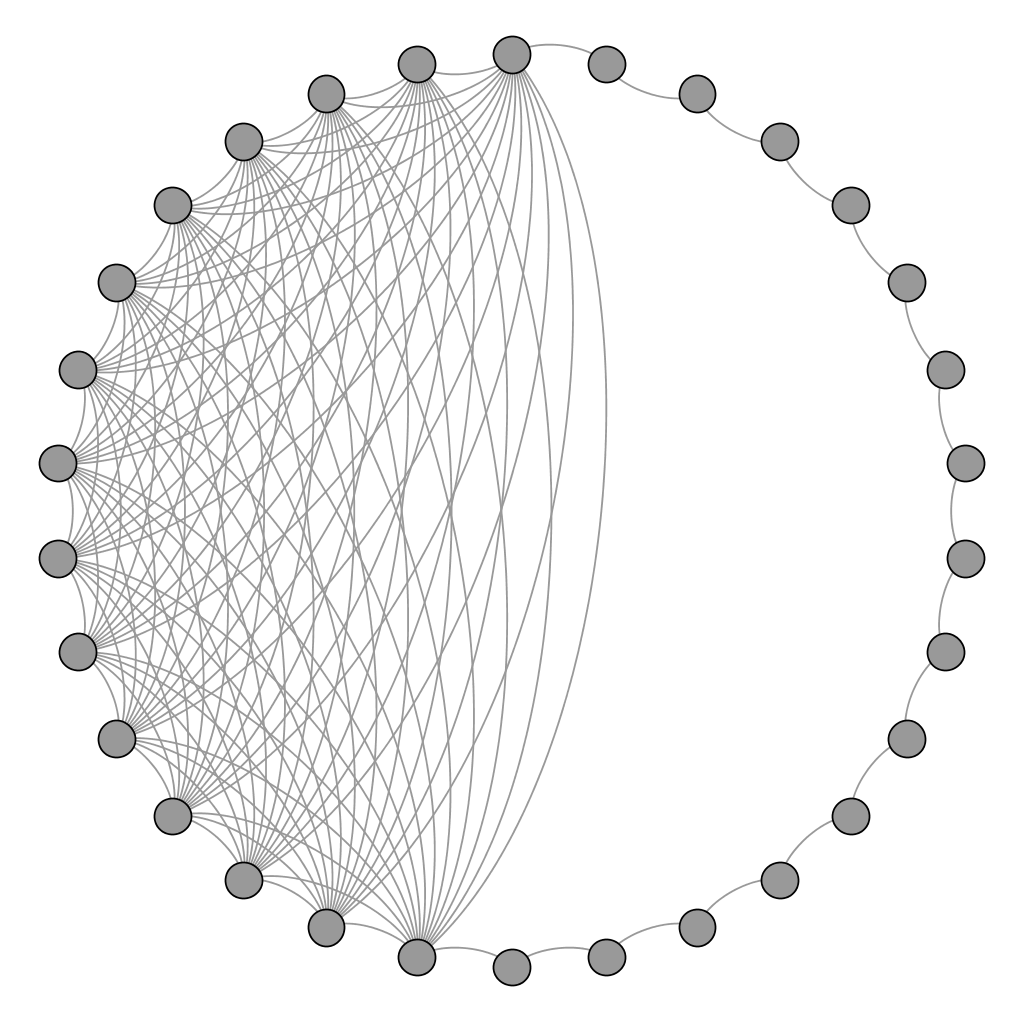
\includegraphics[width=1.0\textwidth, angle=0]{HALFFULLY_CONNECTED_30.png}
	\caption{Half Fully-Connected topology}
	\label{fig1}
\end{figure}

\begin{table}[h]
	\centering
	\caption{Network metrics Half Fully-Connected topology}
	\begin{tabular} { l c r }
		\hline
		Avg. degree & 8.067 \\
		Avg. path-length & 4.007 \\
		Avg. clustering coefficient & 0.491 \\
		Network diameter & 9 \\
		Graph density & 0.278 \\
		\hline
	\end{tabular}
\end{table}

\subsection{Ascending-Connected}
\begin{figure}[H]
	\centering
  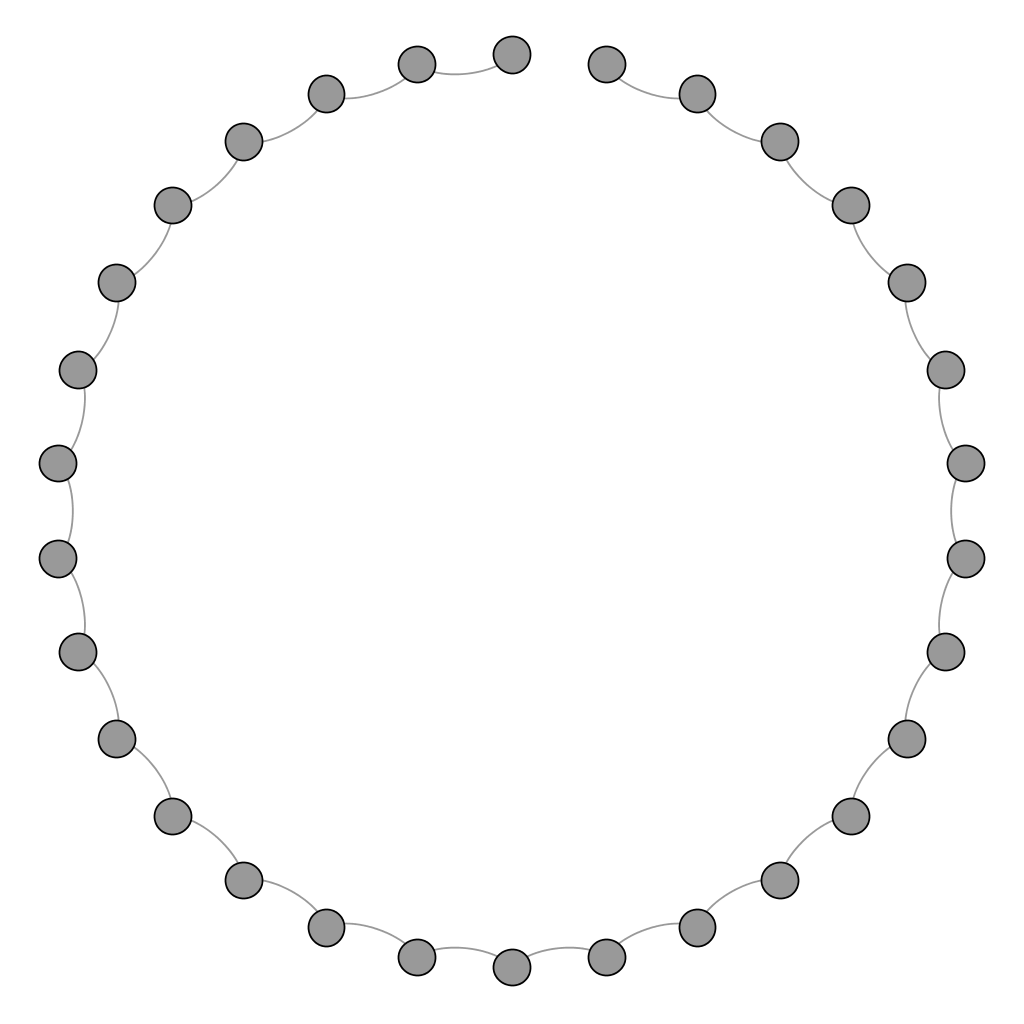
\includegraphics[width=1.0\textwidth, angle=0]{ASCENDING_CONNECTED_30.png}
	\caption{Ascending-Connected topology}
	\label{fig1}
\end{figure}

\begin{table}[h]
	\centering
	\caption{Network metrics Ascending-Connected topology}
	\begin{tabular} { l c r }
		\hline
		Avg. degree & 1.933 \\
		Avg. path-length & 10.33 \\
		Avg. clustering coefficient & 0 \\
		Network diameter & 29 \\
		Graph density & 0.067 \\
		\hline
	\end{tabular}
\end{table}

\subsection{Ascending-Connected with short-cuts}
\subsubsection{Full short-cuts}
\begin{figure}[H]
	\centering
  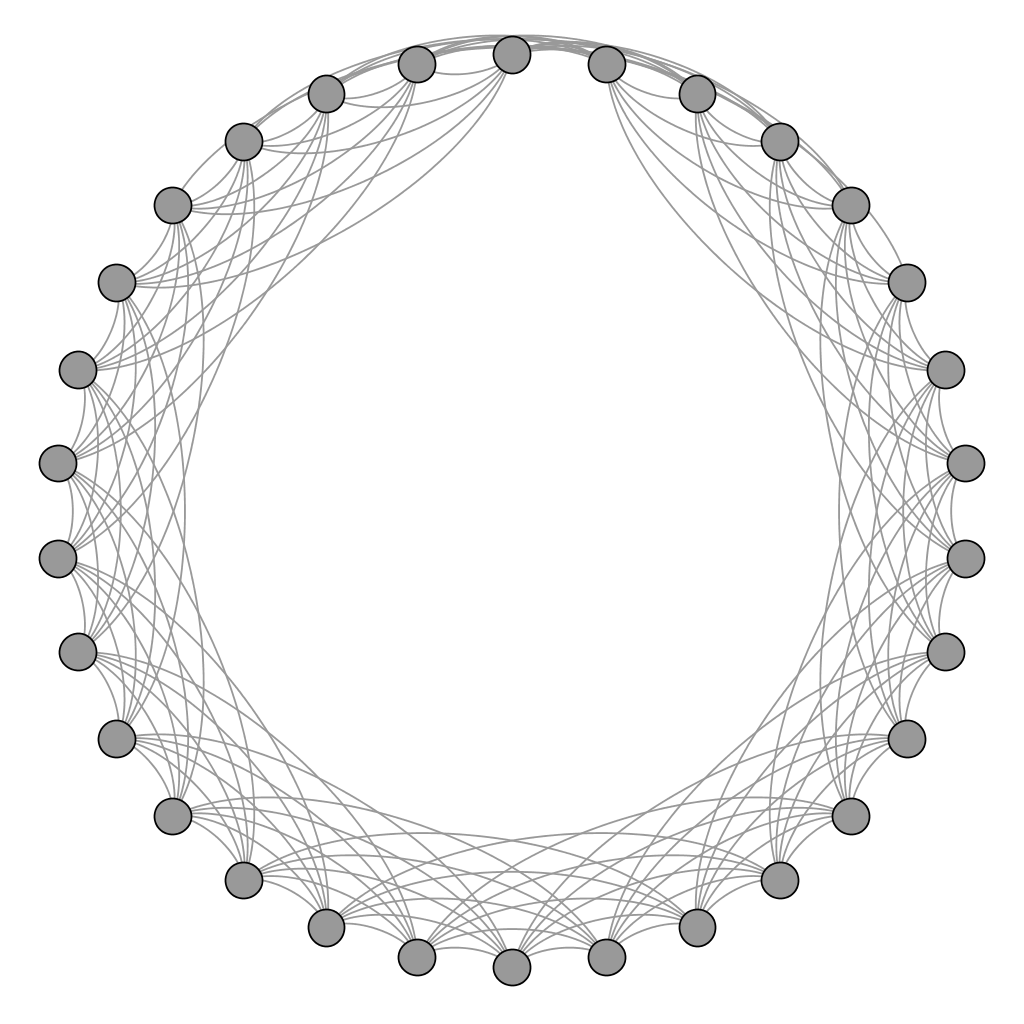
\includegraphics[width=1.0\textwidth, angle=0]{ASCENDING_CONNECTED_FULLSHORTCUTS_5_30.png}
	\caption{Ascending-Connected 5 full short-cuts topology}
	\label{fig1}
\end{figure}

\begin{table}[h]
	\centering
	\caption{Network metrics Ascending-Connected 5 full short-cuts topology}
	\begin{tabular} { l c r }
		\hline
		Avg. degree & 10 \\
		Avg. path-length & 1.966 \\
		Avg. clustering coefficient & 0.667 \\
		Network diameter & 3 \\
		Graph density & 0.345 \\
		\hline
	\end{tabular}
\end{table}

\subsubsection{Regular short-cuts}
\begin{figure}[H]
	\centering
  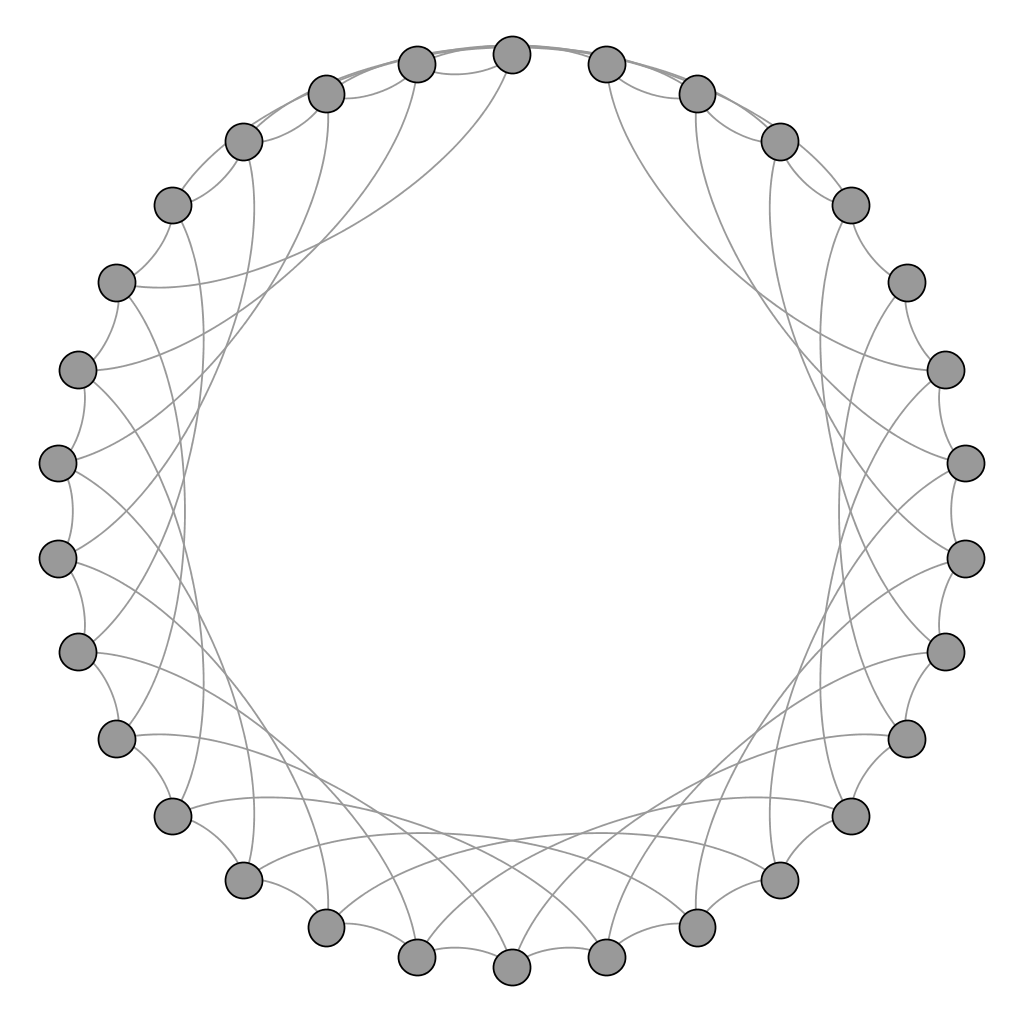
\includegraphics[width=1.0\textwidth, angle=0]{ASCENDING_CONNECTED_REGULARSHORTCUTS_5_30.png}
	\caption{Ascending-Connected 5 regular short-cuts topology}
	\label{fig1}
\end{figure}

\begin{table}[h]
	\centering
	\caption{Network metrics Ascending-Connected 5 regular short-cuts topology}
	\begin{tabular} { l c r }
		\hline
		Avg. degree & 3.867 \\
		Avg. path-length & 2.839 \\
		Avg. clustering coefficient & 0 \\
		Network diameter & 6 \\
		Graph density & 0.133\\
		\hline
	\end{tabular}
\end{table}

\subsubsection{Random short-cuts}
\begin{figure}[H]
	\centering
  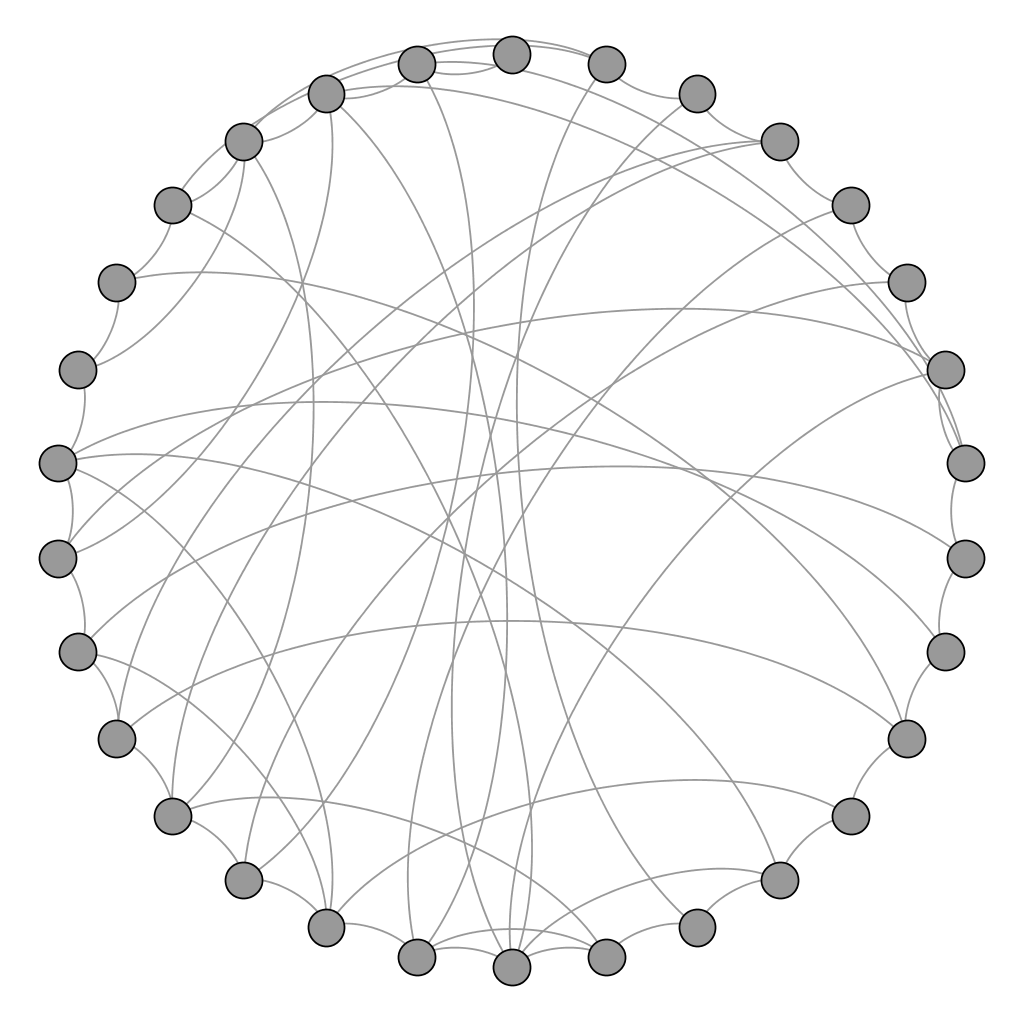
\includegraphics[width=1.0\textwidth, angle=0]{ASCENDING_CONNECTED_RANDOMSHORTCUTS_10_30.png}
	\caption{Ascending-Connected random short-cuts probability 1.0 topology}
	\label{fig1}
\end{figure}

\begin{table}[h]
	\centering
	\caption{Network metrics Ascending-Connected random short-cuts topology}
	\begin{tabular} { l c r }
		\hline
		Avg. degree & 3.867 \\
		Avg. path-length & 2.506 \\
		Avg. clustering coefficient & 0.056 \\
		Network diameter & 5 \\
		Graph density & 0.133\\
		\hline
	\end{tabular}
\end{table}

\subsection{Hub-based topologies}
\subsubsection{3 Hubs}
\begin{figure}[H]
	\centering
  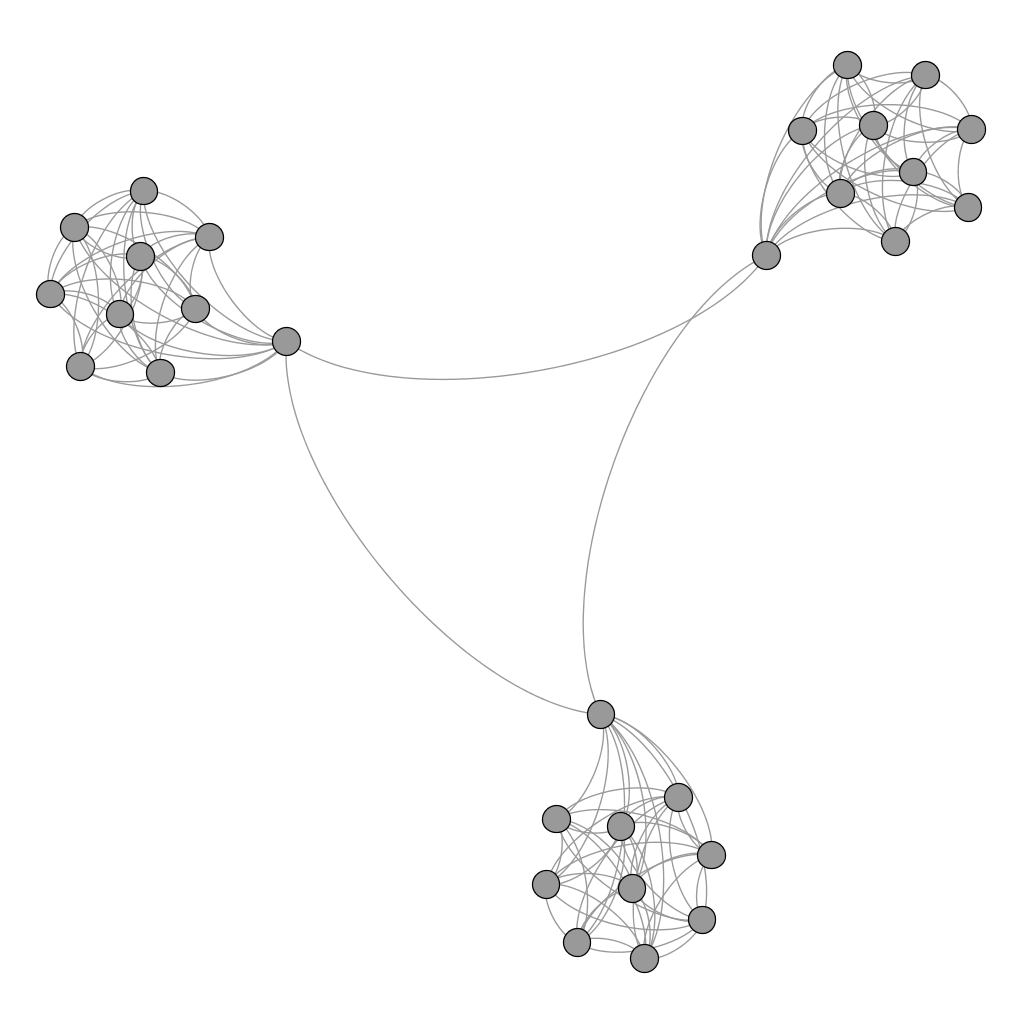
\includegraphics[width=1.0\textwidth, angle=0]{3HUBS_30.png}
	\caption{3 Hubs topology}
	\label{fig1}
\end{figure}

\begin{table}[h]
	\centering
	\caption{Network metrics 3 Hubs topology}
	\begin{tabular} { l c r }
		\hline
		Avg. degree & 9.2 \\
		Avg. path-length & 2.241 \\
		Avg. clustering coefficient & 0.976 \\
		Network diameter & 3 \\
		Graph density & 0.371\\
		\hline
	\end{tabular}
\end{table}

\subsubsection{3 Median Hubs}
\begin{figure}[H]
	\centering
  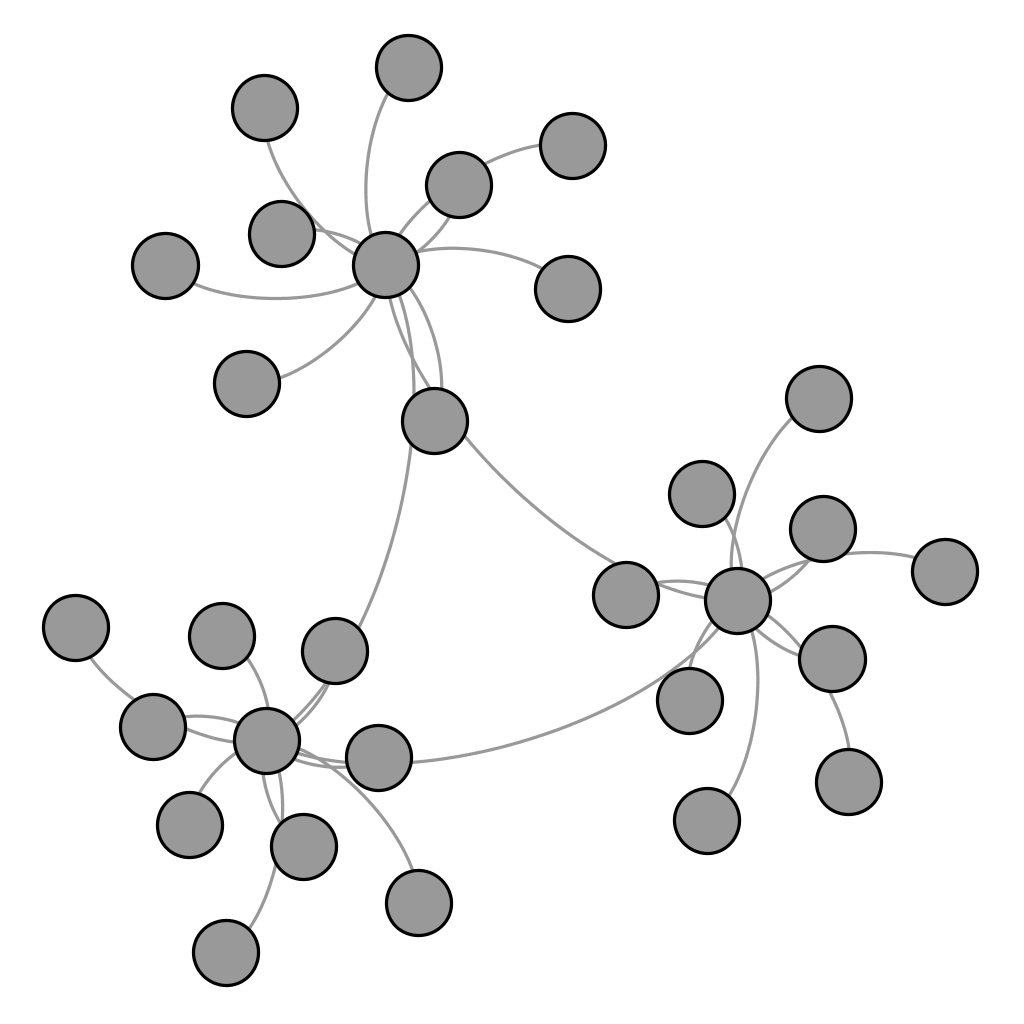
\includegraphics[width=1.0\textwidth, angle=0]{3MEDIANHUB_30.png}
	\caption{3 Median Hub topology}
	\label{fig1}
\end{figure}

\begin{table}[h]
	\centering
	\caption{Network metrics 3 Median Hub topology}
	\begin{tabular} { l c r }
		\hline
		Avg. degree & 2 \\
		Avg. path-length & 2.49 \\
		Avg. clustering coefficient & 0.018 \\
		Network diameter & 3 \\
		Graph density & 0.069 \\
		\hline
	\end{tabular}
\end{table}

\subsubsection{Median Hub}
\begin{figure}[H]
	\centering
  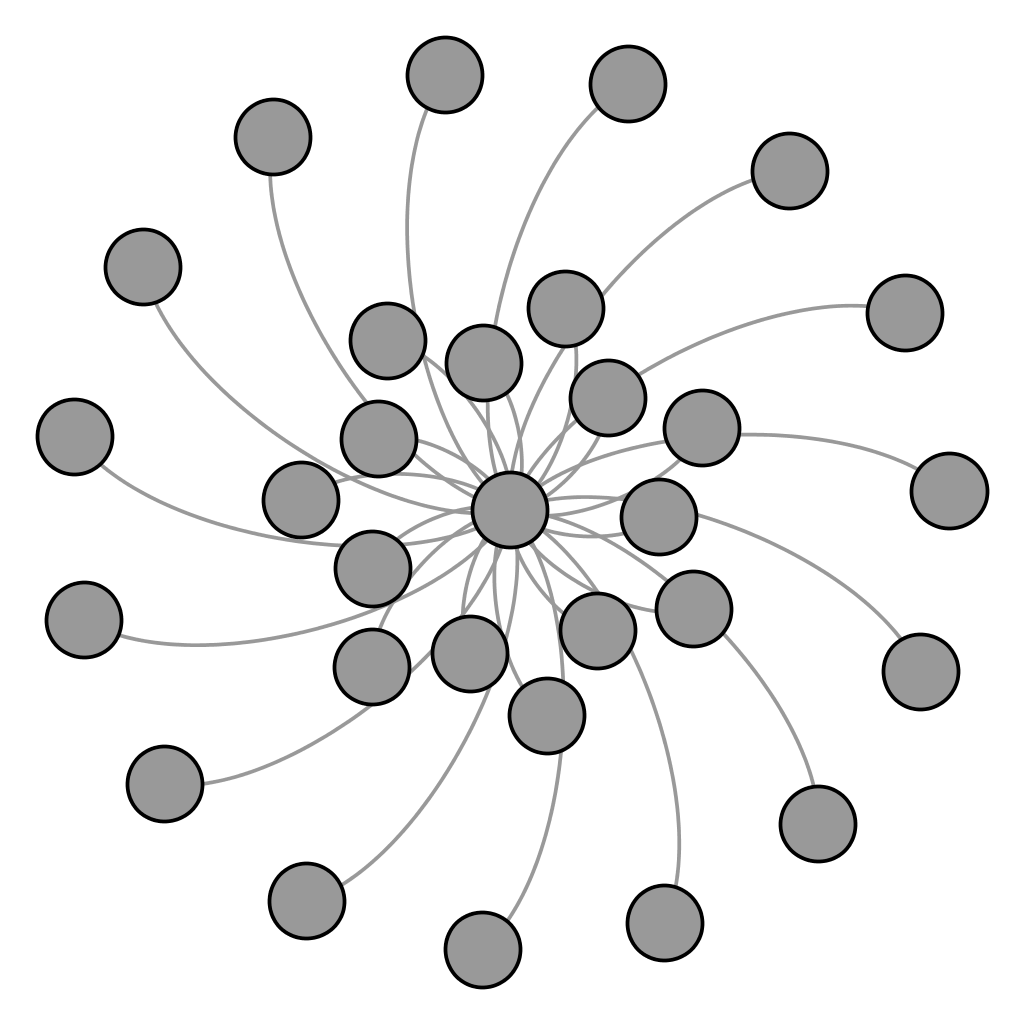
\includegraphics[width=1.0\textwidth, angle=0]{1MEDIANHUB_30.png}
	\caption{Median Hub topology}
	\label{fig1}
\end{figure}

\begin{table}[h]
	\centering
	\caption{Network metrics Median Hub topology}
	\begin{tabular} { l c r }
		\hline
		Avg. degree & 1.933 \\
		Avg. path-length & 1.933 \\
		Avg. clustering coefficient & 0 \\
		Network diameter & 2 \\
		Graph density & 0.067 \\
		\hline
	\end{tabular}
\end{table}

\subsubsection{Maximum Hub}
Looks the same as 1 Median Hub but all edges are connected to the agent with the highest optimism-value.
Has thus also the same metrics as the optimism-values have no functional influence on the metrics.

\subsection{Small-World and Scale-Free topologies}
\subsubsection{Erods-Renyi}

\begin{figure}[H]
	\centering
  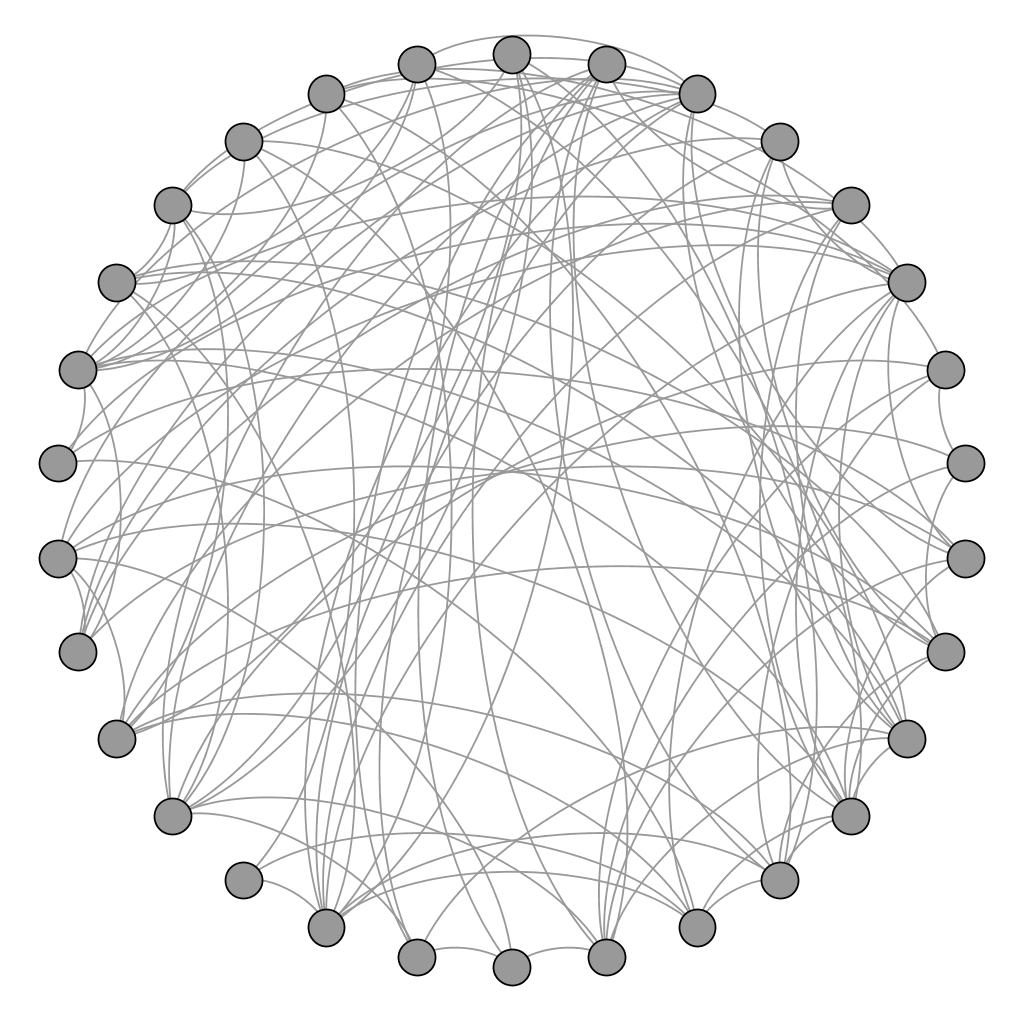
\includegraphics[width=1.0\textwidth, angle=0]{ERDOSRENYI_02_30.png}
	\caption{Erdos-Renyi topology with inclusion-probability of 0.2}
	\label{fig1}
\end{figure}

\begin{table}[h]
	\centering
	\caption{Network metrics Erdosy-Renyi 0.2}
	\begin{tabular} { l c r }
		\hline
		Avg. degree & 6.8 \\
		Avg. path-length & 1.913 \\
		Avg. clustering coefficient &  0.266 \\
		Network diameter & 3 \\
		Graph density & 0.234 \\
		Connected component & 1 \\
		\hline
	\end{tabular}
\end{table}

\begin{figure}[H]
	\centering
  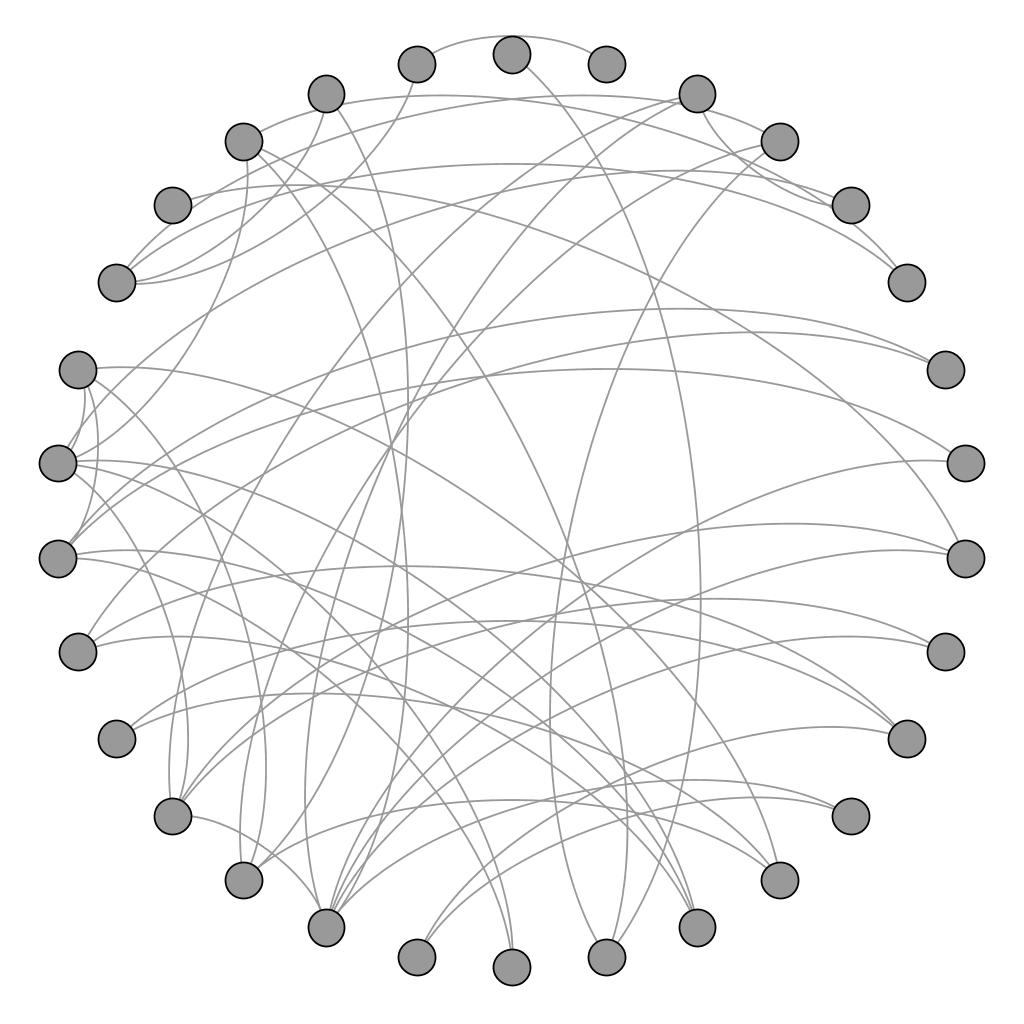
\includegraphics[width=1.0\textwidth, angle=0]{ERDOSRENYI_01_30.png}
	\caption{Erdos-Renyi topology with inclusion-probability of 0.1}
	\label{fig1}
\end{figure}

\begin{table}[h]
	\centering
	\caption{Network metrics Erdosy-Renyi 0.1}
	\begin{tabular} { l c r }
		\hline
		Avg. degree & 2.933 \\
		Avg. path-length & 3.262 \\
		Avg. clustering coefficient & 0.103 \\
		Network diameter & 7 \\
		Graph density & 0.101 \\
		Connected component & 1 \\
		\hline
	\end{tabular}
\end{table}


\begin{figure}[H]
	\centering
  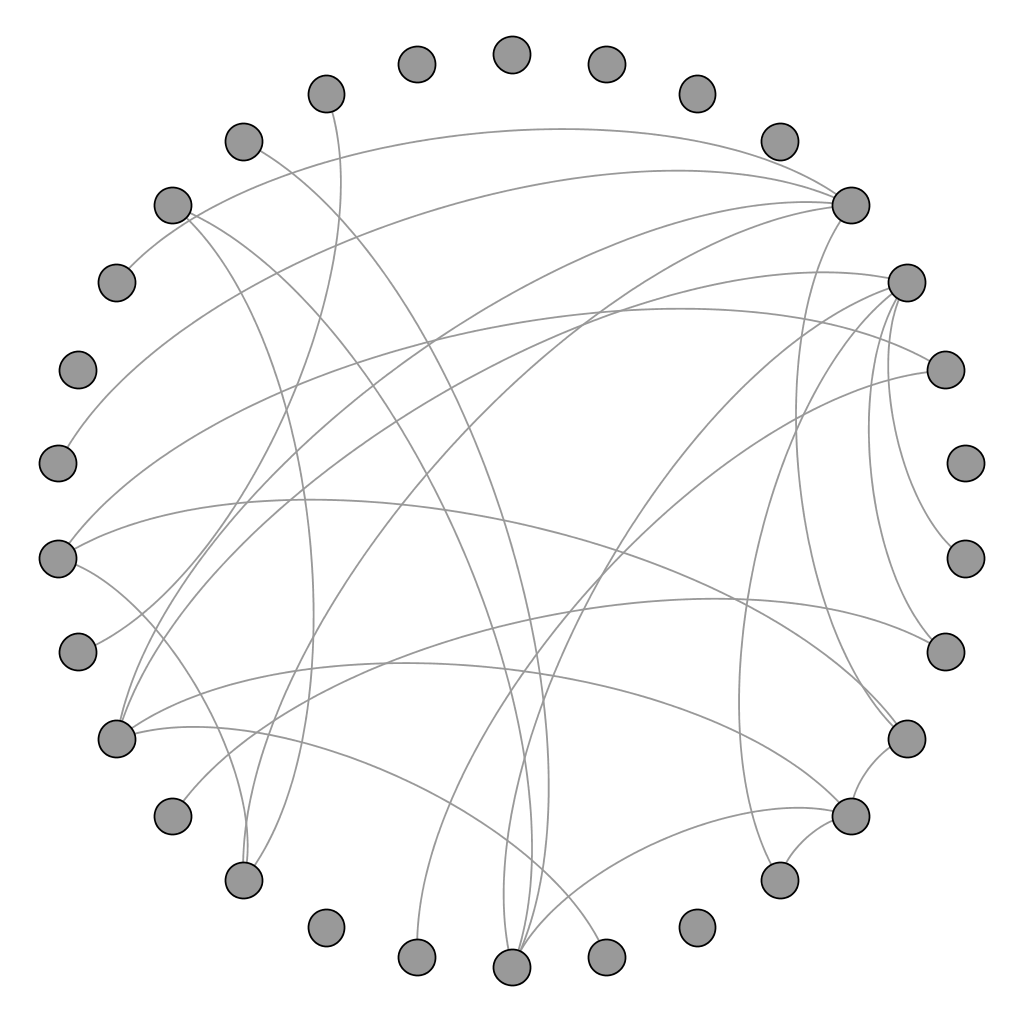
\includegraphics[width=1.0\textwidth, angle=0]{ERDOSRENYI_005_30.png}
	\caption{Erdos-Renyi topology with inclusion-probability of 0.05}
	\label{fig1}
\end{figure}

\begin{table}[h]
	\centering
	\caption{Network metrics Erdosy-Renyi 0.05}
	\begin{tabular} { l c r }
		\hline
		Avg. degree & 1.6 \\
		Avg. path-length & 3.052 \\
		Avg. clustering coefficient & 0 \\
		Network diameter & 8 \\
		Graph density & 0.055 \\
		Connected component & 11 \\
		\hline
	\end{tabular}
\end{table}

\subsubsection{Barbasi-Albert}
\begin{figure}[H]
	\centering
  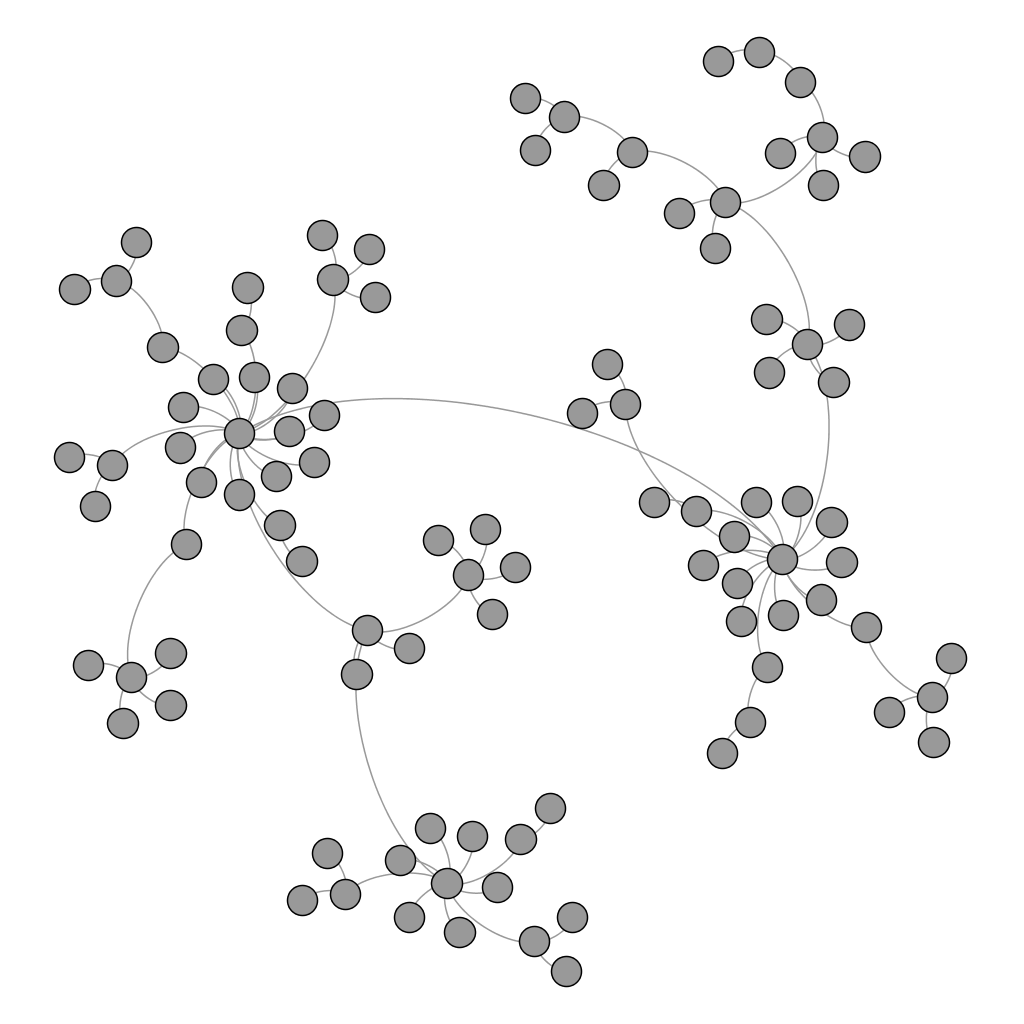
\includegraphics[width=1.0\textwidth, angle=0]{BARBASIALBERT_3_1_30.png}
	\caption{Barbasi-Albert topology with m0=3, m=1}
	\label{fig1}
\end{figure}

\begin{table}[h]
	\centering
	\caption{Network metrics Barbasi-Albert m0=3, m=1}
	\begin{tabular} { l c r }
		\hline
		Avg. degree & 1.98 \\
		Avg. path-length & 4.684 \\
		Avg. clustering coefficient & 0 \\
		Network diameter & 11 \\
		Graph density & 0.02 \\
		\hline
	\end{tabular}
\end{table}

\begin{figure}[H]
	\centering
  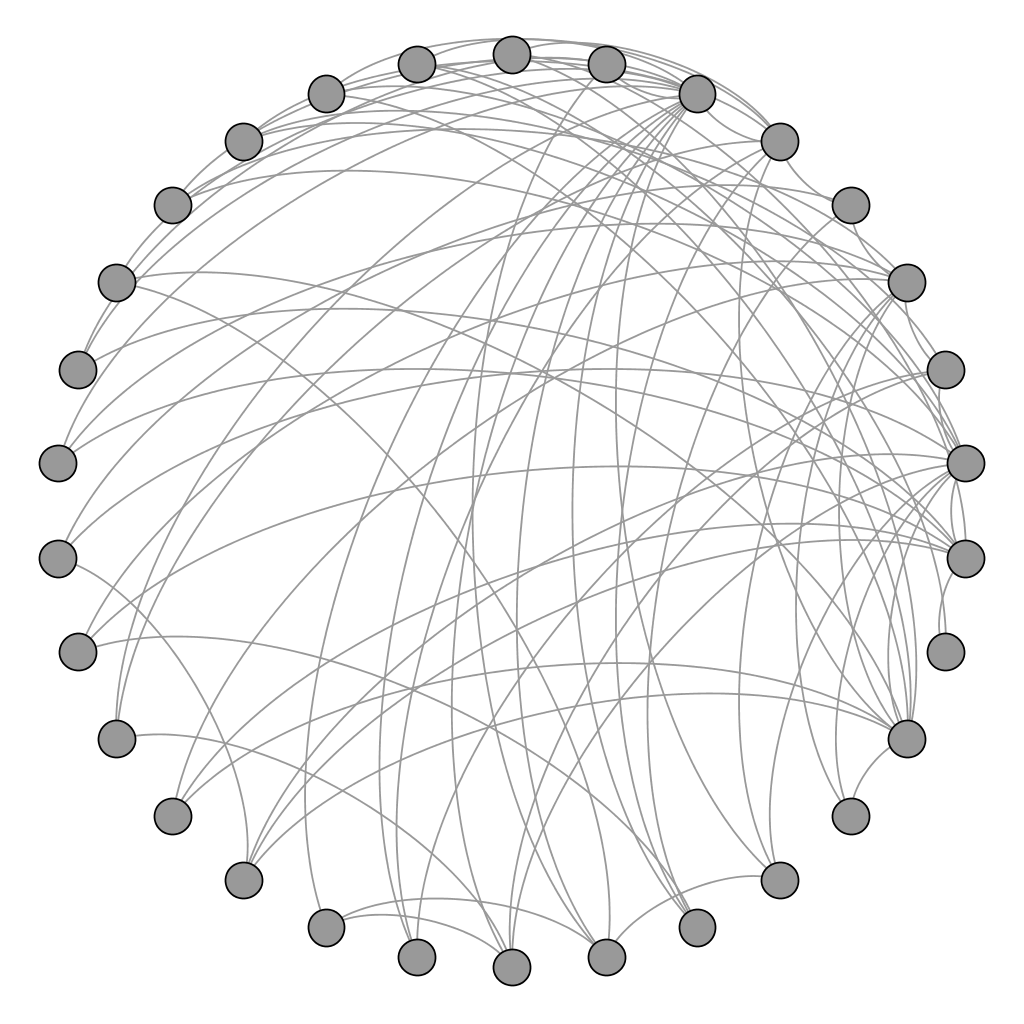
\includegraphics[width=1.0\textwidth, angle=0]{BARBASIALBERT_9_3_30.png}
	\caption{Barbasi-Albert topology with m0=9, m=3}
	\label{fig1}
\end{figure}

\begin{table}[h]
	\centering
	\caption{Network metrics Barbasi-Albert m0=9, m=3}
	\begin{tabular} { l c r }
		\hline
		Avg. degree & 4.733 \\
		Avg. path-length & 2.11 \\
		Avg. clustering coefficient & 0.279 \\
		Network diameter & 4 \\
		Graph density & 0.163 \\
		\hline
	\end{tabular}
\end{table}

\subsubsection{Watts-Strogatz}

Two params: k and p
Creates N nodes and connects each to k neighbours and rewires each then existing edge with a probability of 0.2 to another node with lower id (younger).

\begin{figure}[H]
	\centering
  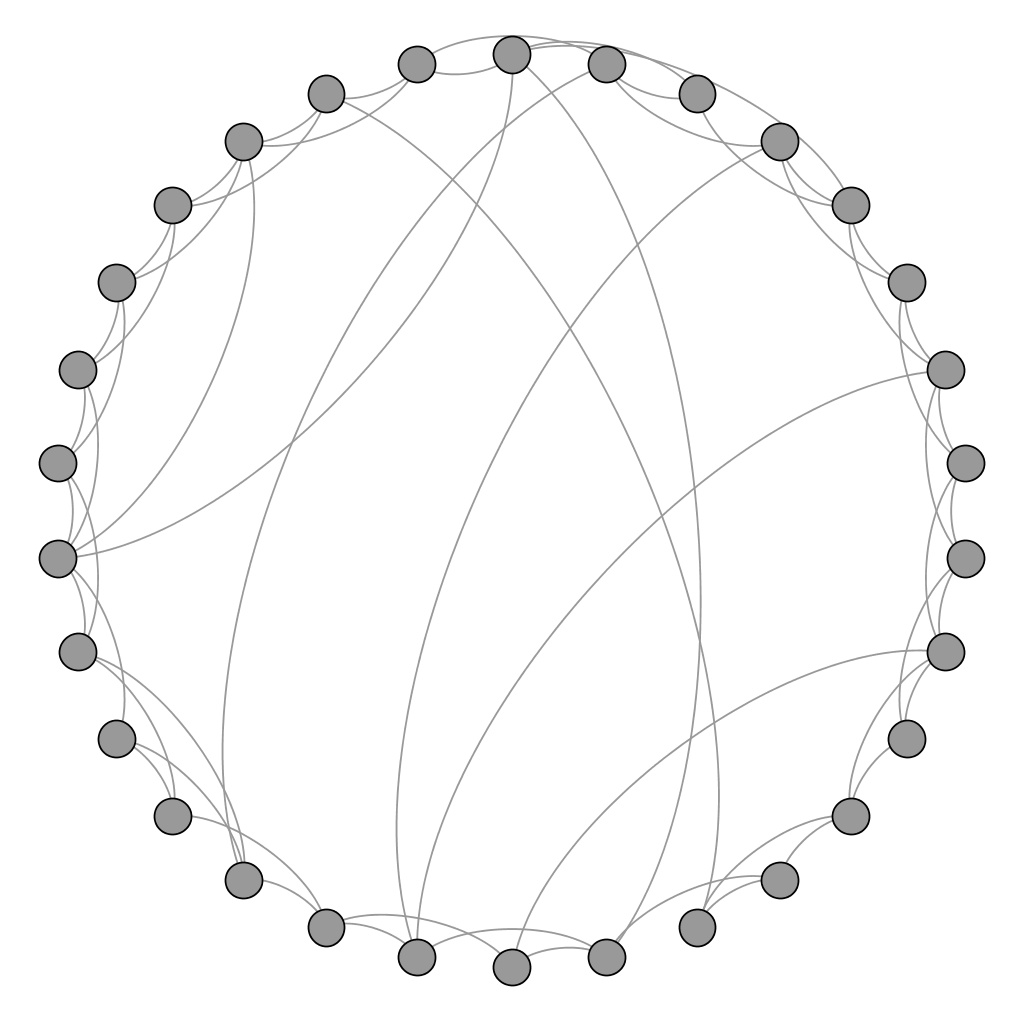
\includegraphics[width=1.0\textwidth, angle=0]{WATTSSTROGATZ_2_02_30.png}
	\caption{Watts-Strogatz topology with k=2, p=0.2}
	\label{fig1}
\end{figure}

\begin{table}[h]
	\centering
	\caption{Network metrics Watts-Strogatz k=2, p=0.2}
	\begin{tabular} { l c r }
		\hline
		Avg. degree & 4 \\
		Avg. path-length & 2.883 \\
		Avg. clustering coefficient & 0.259 \\
		Network diameter & 6 \\
		Graph density & 0.138 \\
		\hline
	\end{tabular}
\end{table}


\begin{figure}[H]
	\centering
  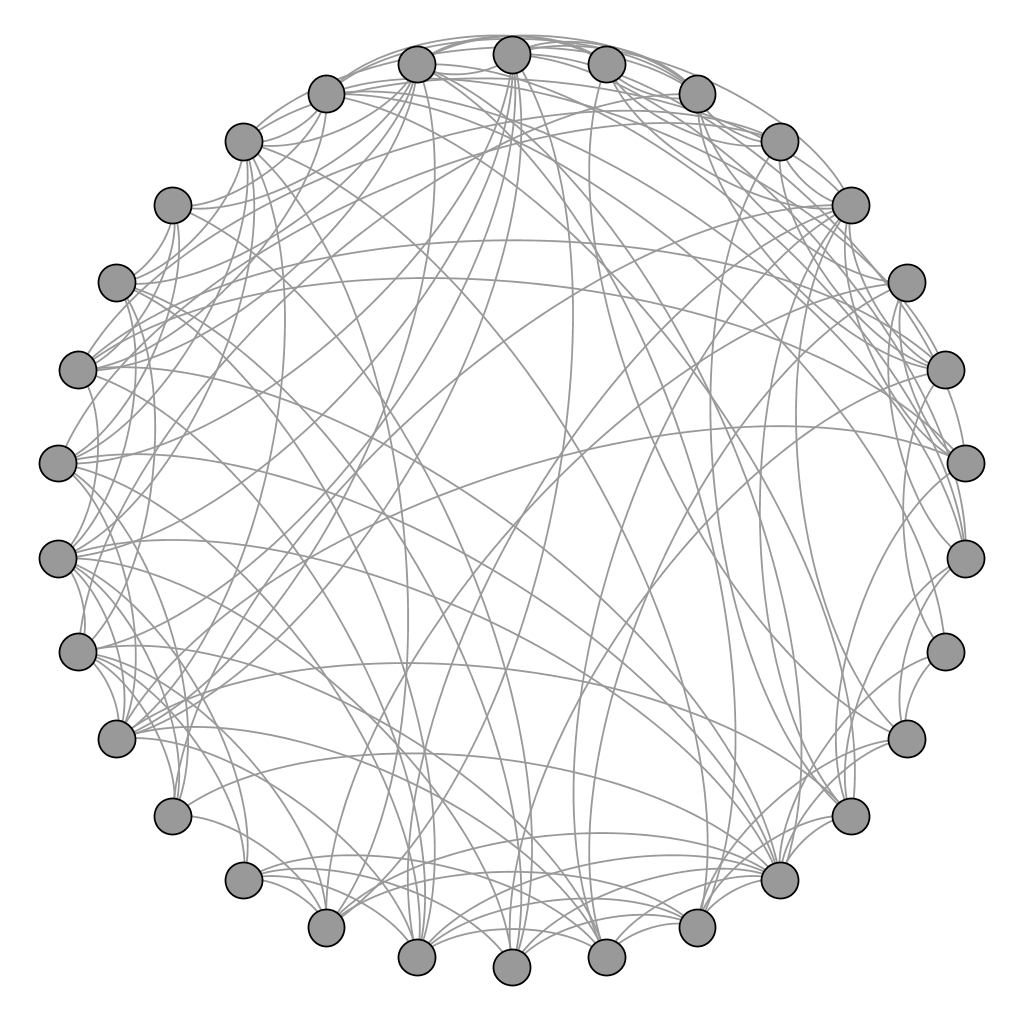
\includegraphics[width=1.0\textwidth, angle=0]{WATTSSTROGATZ_4_05_30.png}
	\caption{Watts-Strogatz topology with k=4, p=0.5}
	\label{fig1}
\end{figure}

\begin{table}[h]
	\centering
	\caption{Network metrics Watts-Strogatz k=4, p=0.5}
	\begin{tabular} { l c r }
		\hline
		Avg. degree & 8 \\
		Avg. path-length & 1.823 \\
		Avg. clustering coefficient & 0.241 \\
		Network diameter & 3 \\
		Graph density & 0.276 \\
		\hline
	\end{tabular}
\end{table}

\end{document}